\documentclass{article}
\usepackage{a4wide}
\usepackage[utf8]{inputenc}
\usepackage{amsmath}
\usepackage{mathtools}
\usepackage{amssymb}
\usepackage[english]{babel}
\usepackage{mdframed}
\usepackage{systeme,}
\usepackage{lipsum}
\usepackage{relsize}
\usepackage{graphicx}
\usepackage{caption}
\usepackage{tikz}
\usepackage{tikz-3dplot}
\usepackage{pgfplots}
\usepackage{harpoon}%
\usepackage{graphicx}
\usepackage{wrapfig}
\usepackage{subcaption}
\usepackage{a4wide}
\usepackage{comment}
\usepackage{authblk}
\usepackage{float}
\usepackage{listings}
\usepackage{xcolor}
\usepackage{amsmath}
\usepackage{chngcntr}
\usepackage{amsthm}
\usepackage{comment}
\usepackage{commath}
\usepackage{hyperref}%Might remove, adds link to each reference
\usepackage{url}
\newcommand{\w}{\omega}
\newcommand{\curl}[1]{\vec{\nabla}\times \vec{#1}}
\newcommand{\grad}{\vec{\nabla}}
\newcommand{\dive}[1]{\vec{\nabla}\cdot \vec{#1}}
%\newcommand{\crr}{\mathfrak{r}}
\usepackage{calligra}

\DeclareMathAlphabet{\mathcalligra}{T1}{calligra}{m}{n}
\DeclareFontShape{T1}{calligra}{m}{n}{<->s*[2.2]callig15}{}
\newcommand{\crr}{\mathcalligra{r}\,}
\newcommand{\boldscriptr}{\pmb{\mathcalligra{r}}\,}

\title{Handin 5}
\author{Author : Andreas Evensen}
\date{Date: \today}
\definecolor{codegreen}{rgb}{0,0.6,0}
\definecolor{codegray}{rgb}{0.5,0.5,0.5}
\definecolor{codepurple}{rgb}{0.58,0,0.82}
\definecolor{backcolour}{rgb}{0.95,0.95,0.92}

\lstdefinestyle{mystyle}{
    backgroundcolor=\color{backcolour},   
    commentstyle=\color{codegreen},
    keywordstyle=\color{magenta},
    numberstyle=\tiny\color{codegray},
    stringstyle=\color{codepurple},
    basicstyle=\ttfamily\footnotesize,
    breakatwhitespace=false,         
    breaklines=true,                 
    captionpos=b,                    
    keepspaces=true,                 
    numbers=left,                    
    numbersep=5pt,                  
    showspaces=false,                
    showstringspaces=false,
    showtabs=false,                  
    tabsize=2
}

\lstset{style=mystyle}

\begin{document}

\maketitle

\section{Warm up}
We wish to integrate the function defined below around a closed countour of radius $3$, centered around the origin.
\begin{align*}
    f(z) = \frac{e^{iz}}{(z^2 + 1)(z + 2)^2}
\end{align*}Firstly we identify the singularities, $z_1 = i$, $z_2 = -i$ and $z_3 = -2$ where the $z_3$ is a double pole. From this we use the Residue theorem, since the function is analytic everywhere except for the singularities in the closed contour.
\begin{comment}
\begin{align*}
    \text{Res}(f, -2) &=\lim_{z\to -2}\frac{d}{dz}\left[\frac{e^{iz}(z+2)^2}{(z-i)(z + i)(z + 2)^2}\right]\\
    &= \frac{9ie^{-2i}}{25}\\
    \text{Res}(f, i) &=\lim_{z\to i}\\
    \text{Res}(f, -i) &=\lim_{z\to i}
\end{align*}
\end{comment}
Thus, one needs only to compute the following residues:
\begin{align*}
    \text{Res}(f, -2) &= \lim_{z\to -2}\frac{1}{2!} \frac{d}{dz}\left[\frac{(z+2)^2e^{iz}}{(z-i)(z+i)(z+2)^2}\right]\\
    &=\lim_{z\to -2}\frac{1}{2}\frac{d}{dz}\left[\frac{e^{iz}}{(z-i)(z+i)}\right]\\
    &=\lim_{z\to-2}\frac{1}{2}\left[\frac{ie^{iz}(z^2 + 1)-2ze^{iz}}{(z^2 + 1)^2}\right]\\
    &=\frac{1}{25}\left(5ie^{-2i} - 4e^{-2i}\right) = \frac{e^{-2i}\big(5i - 4\big)}{25}\\
    \text{Res}(f, i) &=\lim_{z\to i}\frac{e^{iz}(z-i)}{(z-i)(z+i)(z^2 + 2)} = \frac{e^{-1}}{2i}\\
    \text{Res}(f, -i) &=\lim_{z\to i}\frac{e^{iz}(z+i)}{(z-i)(z+i)(z^2 + 2)} = -\frac{e^{1}}{2i}\\
\end{align*}Thus the integral becomes:
\begin{align*}
    \oint f(z)dz &= 2\pi i\cdot\left[\frac{e^{-1}}{2i} - \frac{e^{1}}{2i} + \frac{e^{-2i}\big(5i - 4\big)}{25}\right]\\
    &=\pi e^{-1} - \pi e^{1} + \frac{2\pi e^{-2i}(4i -5)} {25}
\end{align*}
\newpage
\section{Kepler's orbit}
Given the following Lagrangian, one wish to compute the equations of motion for the system:
\begin{align*}
    \mathcal{L} = \frac{1}{2}m_1\dot{\mathbf{r}}_1^2 + \frac{1}{2}m_2\dot{\mathbf{r}}_2^2+ G\frac{m_1m_2}{\abs{\mathbf{r}_1 - \mathbf{r}_2}}
\end{align*}
\subsection*{a)}
Applying the following transformation yeilds:
\begin{align*}
    \begin{cases}
        (m_1 + m_2)\mathbf{R} = m_1\mathbf{r}_1 + m_2\mathbf{r}_2\\
        \mathbf{r} = \mathbf{r}_1 - \mathbf{r}_2
    \end{cases}
\end{align*}
\begin{align*}
    \mathbf{r}_1 &=\text{?}\quad\&\quad \mathbf{r}_2 = \text{?}\\
    &\mathbf{r} + \frac{M}{m_2}\mathbf{R}\\
    &=\mathbf{r}_1+ \frac{m_1\mathbf{r}_1}{m_2}\\
    \implies & \mathbf{r}_1 = \mathbf{R}+\frac{m_2}{M}\mathbf{r}\\
    \implies & \mathbf{r}_2 = \mathbf{R}-\frac{m_1}{M}\mathbf{r}.\\
\end{align*}Hence, the Lagrangian becomes the following in the new coordinates:
\begin{align*}
    \mathcal{L} &= \frac{1}{2}(m_1\dot{\mathbf{r}}_1^2+m_2\dot{\mathbf{r}}_2^2) + G\frac{m_1m_2}{\abs{\mathbf{r}}}\cdot\frac{m_1+m_2}{m_1+m_2}\\
    &=\frac{1}{2}\left(m_1\frac{d}{dt}\left[\mathbf{R}+\frac{m_2}{M}\mathbf{r}\right]^2+m_2\frac{d}{dt}\left[\mathbf{R}-\frac{m_1}{M}\mathbf{r}\right]^2\right) + G\mu \frac{m_1+m_2}{\abs{\mathbf{r}}}\\
    &=\frac{1}{2}\left(m_1\dot{\mathbf{R}}^2 + m_2\dot{\mathbf{R}}^2+m_1\frac{m_2^2}{M^2}\dot{\mathbf{r}}^2 + m_2\frac{m_1^2}{M^2}\dot{\mathbf{r}}^2\right) + \frac{GM\mu}{\abs{\mathbf{r}}}\\
    &=\frac{1}{2}\left[(m_1+m_2)\dot{\mathbf{R}}^2 + \frac{m_1m_2^2+m_2m_1^2}{M^2}\dot{\mathbf{r}}^2\right] + \frac{K}{\abs{\mathbf{r}}}\\
    \mathcal{L} &= \frac{1}{2}M\dot{\mathbf{R}}^2 + \frac{1}{2}\mu\dot{\mathbf{r}}^2 + \frac{K}{\abs{\mathbf{r}}}
\end{align*}
\subsection*{b)}
The four Euler-Lagrange equation:
\begin{equation}\label{eq: 2b lagrangian}
    \mathcal{L} = \frac{1}{2}M\left[\dot{X}\hat{x} + \dot{Y}\hat{y}\right]^2 + \frac{\mu}{2}\frac{d}{dt}\Big(r\cdot\hat{r}(\theta)\Big)^2+\frac{K}{r} 
\end{equation}
\begin{align}
    \frac{d}{dt}\frac{\partial}{\partial \dot{X}}\Big(\mathcal{L}\Big) &=\frac{\partial }{\partial X}\Big(\mathcal{L}\Big)\nonumber\\
    \implies M\ddot{X}&=0\nonumber\\
    \frac{d}{dt}\frac{\partial}{\partial \dot{Y}}\Big(\mathcal{L}\Big)&=\frac{\partial }{\partial Y}\Big(\mathcal{L}\Big)\nonumber\\
    \implies M\ddot{Y}&=0\nonumber\\
    \frac{d}{dt}\frac{\partial}{\partial \dot{r}}\Big(\mathcal{L}\Big) &=\frac{\partial }{\partial r}\Big(\mathcal{L}\Big)\nonumber\\
    \implies\mu\ddot{r}&=r\mu\dot{\theta}^2 - \frac{K}{r^2}\nonumber\\
    \implies\mu\ddot{r}&=\frac{l^2}{\mu r^3} - \frac{K}{r^2}\label{eq: 2b}\\
    \frac{d}{dt}\frac{\partial}{\partial \dot{\theta}}\Big(\mathcal{L}\Big) &=\frac{\partial }{\partial \theta}\Big(\mathcal{L}\Big)\nonumber\\
    \implies \mu \dot{r}^2 &= 0.\nonumber
\end{align}From the Lagrangian defined in eq \eqref{eq: 2b lagrangian} the Euler-lagrange equation for the generalized coordinate $r$ is defined in eq \eqref{eq: 2b}.
The variable $l$ is the thus defined as $l = \mu r^2\dot{\theta}$ and is the angular momentum of the system in these coordinates multiplied buy the effective mass. The center of mass movement of the system is thus $M\ddot{X} + M\ddot{Y} = 0$.

\subsection*{c)}
From eq \eqref{eq: 2b} one expresses $ u = r^{-1}$ which yields the following:
\begin{align*}
    \dot{r} &= \frac{l u^2}{\mu}\frac{d}{d\theta}\Big(\frac{1}{u}\Big) = -\frac{l u^2}{\mu}\frac{du}{d\theta},\\
    \ddot{r} &= -\frac{(l u )^2}{\mu^2}\frac{d^2u}{d\theta^2}.
\end{align*}In the above expression we simply use the fact of the following:
\begin{align*}
    \frac{d}{dt} = \frac{d}{d\theta}\cdot\frac{d\theta}{dt} = \dot{\theta}\frac{d}{d\theta}.
\end{align*}

\subsection*{d)}
The ODE becomes the following:
\begin{align*}
    u'' &= -u - \frac{\mu K}{l^2},\\
    \implies u'' + u &= -\frac{\mu K}{l^2},\\
    \implies u_h(\theta) &= A\cos(\theta) + B\sin(\theta)\\
    \&\quad u_p(\theta) &= -\frac{\mu K}{l^2}\\
    \implies u(\theta) &= A\cos(\theta) + B\sin(\theta) - \frac{\mu K}{l^2} 
\end{align*}
\newpage
\section{Complex potential of a 2D incompressible irrotational flow}

\begin{align}
    \begin{cases}
        u_x = \frac{\partial \phi}{\partial x} = \frac{\partial\psi}{\partial y}\\
        u_y = \frac{\partial \phi}{\partial y} = -\frac{\partial\psi}{\partial x}
    \end{cases}\label{eq: Task 3}
\end{align}
\subsection*{a)}
To show that the function $f(z)$ is holomorphic we need to show that the Cauchy-Riemann equations are satisfied. The Cauchy-Riemann equations are defined as per below:
\begin{align*}
    \frac{\partial \phi}{\partial x} &= \frac{\partial\psi}{\partial y},\\
    \frac{\partial \phi}{\partial y} &= -\frac{\partial\psi}{\partial x}.
\end{align*}From eq \eqref{eq: Task 3} we see that the Cauchy-Riemann equations are satisfied, and thus the function $f(z)$ is holomorphic.
The expression for $f'(z)$ thus becomes:
\begin{align*}
    f'(z) &= \frac{\partial}{\partial x}\Big(\phi(x,y) + i\psi(x,y)\Big)\\
    &=\partial_x\phi + i\partial_x\psi\\
    &= u_x - iu_y
\end{align*}

\subsection*{b)}
One wish to prove the below relationship
\begin{align*}
    \oint f'(z)dz = \oint \mathbf{u}\cdot d\mathbf{l} + i\left[\oint \mathbf{u}\times d\mathbf{l}\right]\cdot \hat{z}
\end{align*}
In order to prove the above relationship we firstly start by computing the integral, using the fact that $\mathbf{u}=\text{curl}(\psi(x,y)\hat{z}) = \partial_y\psi(x,y)\hat{x}-\partial_x\psi(x,y)\hat{y} = u_x\hat{x}+u_y\hat{y}$:
\begin{align*}
    \oint f'(z)dz &= \oint dz\Big(u_x - iu_y\Big)\\
    &=\oint\Big(dx + idy\Big)\Big(u_x - iu_y\Big)\\
    &=\oint \Big(u_x dx -iu_ydx + iu_x dy + u_y dy\Big)\\
    &=\oint \Big(u_x dx + u_y dy\Big) + i \oint \Big(u_xdy - u_ydx \Big)\\
    &=\oint \mathbf{u}\cdot d\mathbf{l} + i\oint \Big(\mathbf{u}\times d\mathbf{l}\Big)\cdot \hat{z}
\end{align*}
This above is the desired result which is obtained using:
\begin{align*}
    \mathbf{u}\times d\mathbf{l} &= \begin{vmatrix}
        \hat{x}&\hat{y}&\hat{z}\\
        u_x&u_y&0\\
        dx&dy&dz
    \end{vmatrix} =\hat{x}u_ydz - \hat{y}u_xdz + \hat{z}u_xdy - \hat{z}u_ydx\\
    \implies (\mathbf{u}\times d\mathbf{l})\cdot \hat{z} &= u_xdy - u_ydx
\end{align*}
\subsection*{c)}
Suppose the following complex functions:
\begin{align}
    f_1(z) &= -i\frac{\Gamma}{2\pi}\log(z)\label{eq: task 3c 1}\\
    f_2(z) &= \frac{\lambda}{2\pi}\log(z)\label{eq: task 3c 2}
\end{align}
In order to compute the flux and the circuation we first need to define the flux and the circulation:
\begin{align*}
   \text{Circulation:}& \quad \oint \mathbf{u}\cdot d\mathbf{l}\\
    \text{Flux:}& \quad \oint \Big(\mathbf{u}\times d\mathbf{l}\Big)\cdot\hat{z}
\end{align*}
In order to compute this we first need to compute the derivative of the complex function $f(z)$, stating that $ z =r e^{i\theta}$:
\begin{align*}
    f_1(r, \theta) &= -i\frac{\Gamma}{2\pi}\log(re^{i\theta})\\
    &=-\frac{\Gamma}{2\pi}\Big(-\theta + i\log(r)\Big)\\
    &=\underbrace{\frac{\Gamma}{2\pi}\theta}_{\phi_1} - i\underbrace{\frac{\Gamma\log(r)}{2\pi}}_{\psi_1}\\
    f_2(r, \theta) &= \frac{\lambda}{2\pi}\log(re^{i\theta})\\
    &=\frac{\lambda}{2\pi}\Big(i\theta + \log(r)\Big)\\
    &=\underbrace{\frac{\lambda}{2\pi}\log(r)}_{\phi_2} + i\underbrace{\frac{\lambda \theta}{2\pi}}_{\psi_2}\\
\end{align*}From this one computes the Cauchy-Riemann equations:
\begin{align}
    \frac{\partial \phi}{\partial r} &= \frac{1}{r}\frac{\partial \psi}{\partial \theta}\label{eq: Riemann 1}\\
    \frac{1}{r}\frac{\partial \phi}{\partial\theta} &= -\frac{\partial \psi}{\partial r}\label{eq: Riemann 2}
\end{align}Using these on the both $f_1$ and $f_2$ yields the following:
\begin{align*}
    f_1(z): \quad 0 &= 0\quad \text{from \eqref{eq: Riemann 1}}\\
    \frac{1}{r}\frac{\Gamma}{2\pi}&=\frac{\Gamma}{2\pi r}\quad \text{from \eqref{eq: Riemann 2}}\\
    \implies \mathbf{u}_1 &= 0\cdot\hat{r} +  \frac{\Gamma}{2\pi r}\hat{\theta}\\
    f_2(z): \quad \frac{\lambda}{2\pi r} &= \frac{\lambda}{2\pi r}\quad \text{from \eqref{eq: Riemann 1}}\\
    0&=0\quad \text{from \eqref{eq: Riemann 2}}\\
    \implies \mathbf{u}_2 &= \frac{\lambda}{2\pi r}\hat{r} + 0\cdot\hat{\theta}
\end{align*}
The circulation integrals now computed for both $f_1$ and $f_2$:
\begin{align*}
    f_1(z):\quad \oint \mathbf{u}_1\cdot d\mathbf{l} &= \oint \frac{\Gamma}{2\pi r}\cdot rd\theta = \Gamma\\
    f_2(z):\quad \oint\mathbf{u}_2\cdot d\mathbf{l} &= \oint \frac{\lambda}{2\pi r}\cdot dr = \frac{\lambda}{2\pi}\ln(r)
\end{align*}
The flux integrals now computed for both $f_1$ and $f_2$:
\begin{align*}
    f_1(z):\quad \oint \Big(\mathbf{u_1}\times d\mathbf{l}\Big)\cdot \hat{z} &= \oint \Big(u_\theta dr + u_r r d\theta\Big)= \frac{\Gamma}{2\pi}\ln(r)\\
    f_2(z):\quad \oint \Big(\mathbf{u_2}\times d\mathbf{l}\Big)\cdot \hat{z} &= \oint \Big(u_\theta dr + u_r r d\theta\Big)= \lambda
\end{align*}
\begin{figure}[H]
    \centering
    \begin{subfigure}[b]{0.45\textwidth}
        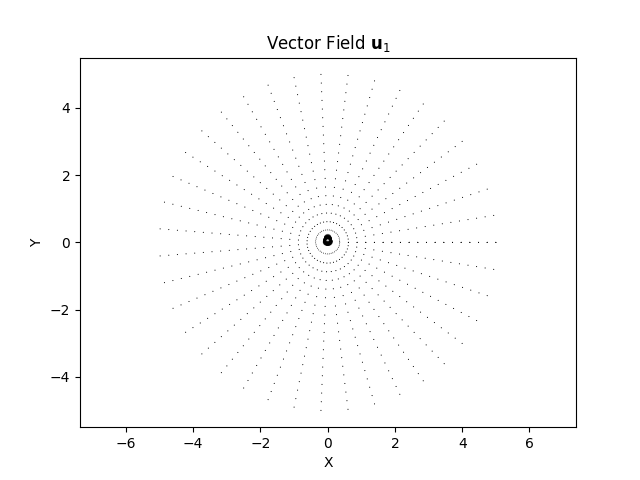
\includegraphics[scale = 0.4]{task3_f1_cir.png}
        \caption{Circulation around the contour for $f_1$.}
        \label{fig:3_2_1}
    \end{subfigure}
    \hfill
    \begin{subfigure}[b]{0.45\textwidth}
        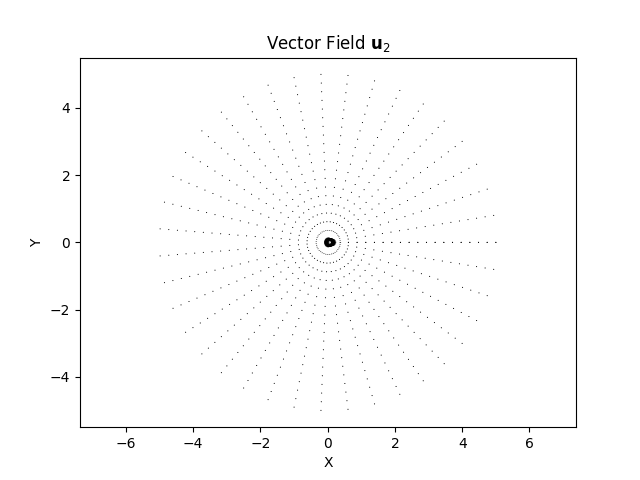
\includegraphics[scale = 0.4]{task3_f2_cir.png}
        \caption{Circulation around the contour for $f_2$.}
        \label{fig:3_2_2}
    \end{subfigure}
    \caption{The velocity fields of $f_1(z)$ and $f_2(z)$.}
\end{figure}\noindent
The figures show the main behavior but are a bit missleading. For $f_1(z)$, the velocity fields curves itself around the origin, and for $f_2(z)$ the velocity field is expanding outwards.
\subsection*{d)}
One applies Stokes theorem to the circulation integral:
\begin{align*}
    &\oint_{\partial \Pi} \mathbf{u}\cdot d\mathbf{l}\quad \text{Stokes' theorem}\\
    \implies &\iint_{\Pi} (\nabla\times \mathbf{u})\cdot d\mathbf{S}.
\end{align*}Due to the definition of $u$, $\nabla \times \mathbf{u}=\mathbf{0}$ and thus the circulation is irrotational.

\newpage
\section{Solving an inhomogeneous ODE using Green’s functions}
\begin{align}
    y''(x) + 4y(x) =\exp\left[\frac{x}{2}\right]; \quad y(0) = y\left(\frac{\pi}{4}\right) = 0\label{eq: Task 4}
\end{align}
\subsection*{a)}
An self-adjoint equation is an equation where the operator of which is acting on the equation is self-adjoint. An example on such an equation would be Schrödingers equation, where the differential operator is defined by:
\begin{align*}
    \hat{H} = -\frac{\hbar^2}{2m}\nabla^2 + V(\mathbf{r}),
\end{align*}The hamiltonian $\hat{H}$ is an self-adjoint operator and when acting on a wave-function $\psi$ it will yeild an self-adjoint equation. Homogenous boundary conditions means that the boundary conditions are equal to zero, and inhomogenous boundary conditions means that the boundary conditions are not equal to zero, either Dirchlet boundary conditions, Neumann or Robin boundary conditions.\\\\
\noindent
Two major restriction on the Green's function is that is has to be piece-wise smooth, and that it must obey the boundary conditions. If the boundary conditions are inhomogeneous the Green's function will be inhomogeneous as well, and thus one can not state
that the Green's function is piece-wise smooth.

\subsection*{b)}
Firstly, we state that the solution $y$ can be written as a linear combination of two functions $y_1$ and $y_2$, where one is the homogenous solution and the other is the particular solution.
\begin{align*}
    \frac{d}{dx}\left[p(x)\frac{dy}{dx}\right] + q(x)y(x) &= f(x)\\
    y''(x) + 4y(x) &= \exp\left[\frac{x}{2}\right]\\
\end{align*}The differential operator $\mathcal{L}$ is thus defined as per below, and the Green's function $\mathcal{G}$ is defined as the solution to the equation below:
\begin{align*}
    \mathcal{L} &= \frac{d^2}{dx^2} + 4\\
    \mathcal{L}y &= y''(x) + 4y(x)\\
    \mathcal{L}\mathcal{G}(x, s) &= \delta(x - s)\\
\end{align*}Applying the Green's function yields:
\begin{align*}
    \frac{d^2}{dx^2}\mathcal{G}(x,s) + 4\mathcal{G}(x,s) &= 0\quad \forall x\neq s\\
    \implies \mathcal{G}(x,s) &= A\sin(2x) + B\cos(2x)\\
    \mathcal{G}_1(x,s) &= A_1\cos(2x) + B_2\sin(2x)\\
    \mathcal{G}_2(x,s) &= A_2\cos(2x) + B_2\sin(2x)\\
\end{align*}From the boundary conditions we limit the coefficients $A_i$ and $B_i$:
\begin{align*}
    \mathcal{G}_1(0,s) &= A_1\cos(0) + B_1\sin(0)\implies A_1 = 0\\
    \mathcal{G}_2\Big(\frac{\pi}{4},s\Big) &= A_2\cos\Big(\frac{\pi}{2}\Big) + B_2\sin\Big(\frac{\pi}{2}\Big)\implies B_2 = 0\\
    \mathcal{G}(x,s) &= \mathcal{G}_1 +\mathcal{G}_2 = B_1\sin(2x) + A_2\cos(2x)\\
\end{align*}The continuity condition, and the jump-condition yields the following:
\begin{align*}
    &\mathcal{G}_1(s,s) = \mathcal{G}_2(s,s),\\
    &B_1\sin(2s) = A_2\cos(2s)\\
    \implies B_1 &= A_2\cot(2s)\\
    &\frac{d\mathcal{G}_2}{dx}\Big|_{x = s} - \frac{d\mathcal{G}_1}{dx}\Big|_{x = s} = \frac{1}{p(x)} = 1\\
    & -2A_2\sin(2s) - 2B_1\cos(2s) = 1\\
    &-2A_2\Big(\sin(2s) + \cot(2s)\cos(2s)\Big) = 1\\
    &-2A_2\Big(\frac{\sin^2(2s) + \cos^2(2s)}{\sin(2s)}\Big)=1\\
    \implies & A_2 = -\frac{1}{2}\sin(2s)\\
    \implies & B_1 = -\frac{1}{2}\cot(2s)\sin(2s) = -\frac{1}{2}\cos(2s)\\
    \implies \mathcal{G} &= \begin{cases}
        -\frac{1}{2}\sin(2s)\cos(2x); \quad x\in[0,s)\\
        -\frac{1}{2}\cos(2s)\sin(2x); \quad x\in(s,\frac{\pi}{4}]
    \end{cases}
\end{align*}
Applying the Green's function to the inhomogeneous equation yields the following:
\begin{align*}
   y_p(x) &=\int_0^L \mathcal{G}(x,s)f(s)ds\\
    &= \int_0^x ds\Big(\mathcal{G}_1(x,s)f(s)\Big) + \int_x^{L} ds\Big(\mathcal{G}_2(x,s)f(s)\Big)\\
    &= \frac{-\cos(2x)}{2}\int_0^x ds\Big(\sin(2s)e^{\frac{s}{2}}\Big) + \frac{-\sin(2x)}{2}\int_x^{L} ds\Big(\cos(2s)e^{\frac{s}{2}}\Big)\\
    &= \frac{-\cos(2x)}{2\cdot 2i}\int_0^x ds\left[\Big(e^{i2s} - e^{-i2s})e^{\frac{s}{2}}\right] + \frac{-\sin(2x)}{2\cdot 2}\int_x^{L} ds\left[\Big(e^{i2s} + e^{-i2s}\Big)e^{\frac{s}{2}}\right]\\
    &= \frac{-\cos(2x)}{2\cdot 2i}\int_0^x ds\left[e^{s (2i + \frac{1}{2})} - e^{s(-2i + \frac{1}{2})}\right] + \frac{-\sin(2x)}{2\cdot 2}\int_x^{L} ds\left[e^{s(2i + \frac{1}{2})} + e^{s(-2i + \frac{1}{2})}\right]\\
    &=-\frac{\cos(2x)}{4i}\left[\frac{e^{s(2i +\frac{1}{2})}}{2i + \frac{1}{2}}- \frac{e^{s(-2i + \frac{1}{2})}}{-2i + \frac{1}{2}}\right]_{s = 0}^{x} - \frac{\sin(2x)}{4}\left[\frac{e^{s(2i + \frac{1}{2})}}{2i + \frac{1}{2}} + \frac{e^{s(-2i + \frac{1}{2})}}{-2i +\frac{1}{2}}\right]_{s = x} ^{\frac{\pi}{4}}\\
    &=-\frac{\cos(2x)}{4i}\left[\frac{e^{x(2i + 0.5)}}{2i + 0.5} - \frac{e^{x(-2i+0.5)}}{-2i + 0.5} - \frac{1}{2i + 0.5} + \frac{1}{(-2i + 0.5)}\right]\\
    &-\frac{\sin(2x)}{4}\left[\frac{e^{\frac{\pi}{4}(2i + 0.5)}}{2i + 0.5} - \frac{e^{\frac{\pi}{4}(-2i + 0.5)}}{-2i + 0.5} - \frac{e^{x(2i + 0.5)}}{2i + 0.5} + \frac{e^{x(-2i + 0.5)}}{-2i + 0.5}\right]
\end{align*}
The homogenous solution is determined by the following:
\begin{align*}
    y_h'' + 4y_h &= 0\\
    \implies y_h(x) &= A\cos(2x) + B\sin(2x),\\
\end{align*}The total solution thus becomes:
\begin{align*}
    y(x) &= A\cos(2x) + B\sin(2x) + -\frac{\cos(2x)}{4i}\left[\frac{e^{x(2i + 0.5)}}{2i + 0.5} - \frac{e^{x(-2i+0.5)}}{-2i + 0.5} - \frac{1}{2i + 0.5} + \frac{1}{(-2i + 0.5)}\right]\\
    &-\frac{\sin(2x)}{4}\left[\frac{e^{\frac{\pi}{4}(2i + 0.5)}}{2i + 0.5} - \frac{e^{\frac{\pi}{4}(-2i + 0.5)}}{-2i + 0.5} - \frac{e^{x(2i + 0.5)}}{2i + 0.5} + \frac{e^{x(-2i + 0.5)}}{-2i + 0.5}\right] 
\end{align*}

\end{document}
    